\chapter{Обработчик прерывания от системного таймера в системах разделения времени}

%Тик -- период времени между двумя последовательными прерываниями системного таймера. В системах UNIX продолжительность тика обычно составляет 10 миллисекунд.

%Основной тик -- период времени равный $n$ тикам системного таймера. Число $n$ зависит от конкретного варианта системы.

%Квант -- период времени, выделенный планировщиком, в течение которого процесс может выполняться.

\section{UNIX-системы}

В UNIX-системах обработчик прерывания от системного таймера \textbf{по тику} выполняет следующие задачи:

\begin{itemize}
	\item инкремент счётчика тиков;
	\item обновление статистики использования процессора текущим процессом;
	\item пересчёт часов, минут и секунд;
	\item декремент счётчика тиков до отправления на выполнение отложенных вызовов, и установка флага для обработчика отложенных вызовов при достижении этим счётчиком нуля.
\end{itemize}

\textbf{По главному тику} обработчик прерывания от системного таймера выполняет ниже перечисленные задачи:

\begin{itemize}
	\item регистрацию отложенных вызовов функций, относящихся к работе планировщика, таких как пересчёт приоритетов процессов;
	\item пробуждение в нужные моменты системных процессов, таких как \textbf{swapper} и \textbf{pagedaemon} (пробуждение означает регистрацию отложенного вызова процедуры \textbf{wakeup}, которая помещает дескриптор процесса в очередь готовых к выполнению процессов);
	\item декремент счётчика времени, оставшегося до посылки одного из следующих сигналов:
	\begin{itemize}[$\bullet$]
		\item \textbf{SIGALRM} -- сигнал, посылаемый процессу по истечении заданного времени функцией \textbf{alarm};
		\item \textbf{SIGPROF} -- сигнал, посылаемый процессу по истечении времени заданного в таймере профилирования;
		\item \textbf{SIGVTALRM} -- сигнал, посылаемый процессу по истечении времени, заданного <<виртуальным>> таймером.
	\end{itemize}
\end{itemize}

\textbf{По кванту} обработчик прерывания выполняет следующую задачу:

\begin{itemize}
	\item посылает текущему процессу сигнал \textbf{SIGXCPU}, если он превысил лимит процессорного времени.
\end{itemize}

\section{Windows-системы}

Обработчик прерывания от системного таймера \textbf{по тику} выполняет следующие задачи:

\begin{itemize}
	\item инкремент счётчика тиков;
	\item декремент остатка кванта текущего потока;
	\item декремент счетчика отложенных задач;
	\item постановка в очередь DPC объекта диспетчера настройки баланса (этот диспетчер активизируется каждую секунду для возможной инициации событий, связанных с планированием и управлением памятью).
\end{itemize}

\textbf{По главному тику} обработчик прерывания выполняет следующее действие:

\begin{itemize}
	\item возвращает задействованный в системе объект <<событие>>, который ожидает диспетчер настройки баланса.
\end{itemize}

\textbf{По кванту} обработчик прерывания от системного таймера выполняет следующую задачу:

\begin{itemize}
	\item инициализирует диспетчеризацию потоков путем постановки соответствующего объекта в очередь DPC.
\end{itemize}

\chapter{Пересчёт приоритетов}

\section{UNIX-системы}

Очередь готовых к выполнению процессов формируется согласно приоритетам процессов и принципу вытесняющего циклического планирования: процессы с одинаковыми приоритетами выполняются в течении кванта времени циклически друг за другом. Если процесс, имеющий более высокий приоритет, поступает в очередь готовых к выполнению, планировщик вытесняет текущий процесс и предоставляет ресурс более приоритетному.

В современных системах Unix ядро является вытесняющим -- процесс в режиме ядра может быть вытеснен более приоритетным процессом в режиме ядра.

\subsection{Приоритеты процессов}

Приоритет процесса в UNIX задаётся числом в диапазоне от 0 до 127, причём чем меньше значение, тем выше приоритет. Приоритеты 0-49 зарезервированы ядром операционной системы, прикладные процессы могут обладать приоритетом в диапазоне от 50 до 127.

Приоритеты ядра являются фиксированными величинами. Приоритеты прикладных задач могут изменяться во времени в зависимости от следующих двух факторов:

\begin{itemize}
	\item фактор любезности – целое число в диапазоне от -20 до 19. Чем меньше значение фактора любезности, тем выше приоритет процесса. Фактор любезности процесса может быть изменён суперпользователем системным вызовом nice;
	\item степень загруженности процессора в момент последнего обслуживания им процесса.
\end{itemize}

Структура \textbf{proc} содержит следующие поля, относящиеся к приоритетам:

\begin{itemize}
	\item \textbf{p\_pri} – текущий приоритет планирования;
	\item \textbf{p\_usrpri} – приоритет режима задачи;
	\item \textbf{p\_cpu} – результат последнего измерения использования процессора;
	\item \textbf{p\_nice} – показатель уступчивости, устанавливаемый пользователем.
\end{itemize}

Планировщик использует поле p\_pri для принятия решения о том, какой процесс отправить на выполнение. Значения p\_pri и p\_usrpri одинаковы, когда процесс находится в режиме задачи. Когда процесс просыпается после блокировки в системном вызове, его приоритет временно повышается. Планировщик использует p\_usrpri для хранения приоритета, который будет назначен процессу при переходе из режима ядра в режим задачи, а p\_pri – для хранения временного приоритета для выполнения в режиме ядра.

Ядро связывает приоритет сна (0-49) с событием или ожидаемым ресурсом, из-за которого процесс может быть заблокирован. Когда блокированный процесс просыпается, ядро устанавливает p\_pri, равное приоритету сна события или ресурса, на котором он был заблокирован, следовательно, такой процесс будет назначен на выполнение раньше, чем другие процессы в режиме задачи.

В таблице \ref{table:1} приведены значения приоритетов сна для систем 4.3BSD UNIX и SCO UNIX. Такой подход позволяет системным вызовам быстрее завершать свою работу. По завершении процессом системного вызова его приоритет сбрасывается в значение текущего приоритета в режиме задачи. Если при этом приоритет окажется ниже, чем приоритет другого запущенного процесса, ядро произведет переключение контекста.

\begin{table}
	\begin{center}
		\caption{Таблица приоритетов в системе 4.3BSD}
		\begin{tabular}{|c|c|c|}
			\hline
			\textbf{Приоритет} & \textbf{Значение} & \textbf{Описание} \\
			\hline
			PSWP & 0 & Своппинг \\
			PSWP + 1 & 1 & Страничный демон \\
			PSWP + 1/2/4 & 1/2/4 & Другие действия по обработке памяти \\
			\hline
			PINOD & 10 & Ожидание освобождения inode \\
			PRIBIO & 20 & Ожидание дискового ввода-вывода \\
			PRIBIO + 1 & 21 & Ожидание освобождения буфера \\
			\hline
			PZERO & 25 & Базовый приоритет \\
			TTIPRI & 28 & Ожидание ввода с терминала \\
			TTOPRI & 29 & Ожидание вывода в терминал \\
			\hline
			PWAIT & 30 & Ожидание завершения процесса-потомка \\
			PLOCK & 35 & Ожидание блокированного ресурса \\
			PSLEP & 40 & Ожидание сигнала \\
			\hline
		\end{tabular}
		\label{table:1}
	\end{center}
\end{table}

\clearpage

Приоритет в режиме задачи зависит от уступчивости и последней измеренной величины использования процессора. Степень уступчивости – это число в диапазоне от -20 до 19 со значением 0 по умолчанию.

Системы разделения времени стараются выделить процессорное время таким образом, чтобы все процессы системы получили его в равных количествах, что требует слежения за использованием процессора. Поле p\_cpu содержит величину последнего измерения использования процессора процессом. При создании процесса это поле инициализируется нулем. На каждом тике обработчик таймера увеличивает p\_cpu на единицу для текущего процесса, вплоть до максимального значения – 127. Каждую секунду ядро вызывает процедуру schedcpu, которая уменьшает значение p\_cpu каждого процесса исходя из фактора <<полураспада>>.

В 4.3BSD для расчета применяется формула

\begin{equation}
decay = \frac{2*load\_average}{2*load\_average + 1},
\end{equation}

где load\_average -- это среднее количество процессов, находящихся в состоянии готоврости к выполнению за последнюю секунду.

Кроме того, процедура schedcpu также пересчитывает приоритеты режима задачи всех процессов по формуле

\begin{equation}
p\_usrpri = PUSER + \frac{p\_cpu}{4} + 2*p\_nice,
\end{equation}

где PUSER -- базовый приоритет в режиме задачи, равный 50.

Если процесс до вытеснения другим процессом использовал большое количество процессорного времени, его p\_cpu будет увеличен, что приведет к увеличению значения p\_usrpri и к понижению приоритета. Чем дольше процесс простаивает в очереди на выполнение, тем меньше его p\_cpu. Это позволяет предотвратить зависания низкоприоритетных процессов. Если процесс б$\acute{\textrm{о}}$льшую часть времени выполнения тратит на ожидание ввода-вывода, то он остается с высоким приоритетом.

Системы разделения времени пытаются выделить процессорное время таким образом, чтобы конкурирующие процессы получили его примерно в равных количествах. Фактор полураспада обеспечивает экспоненциально взвешанное среднее значение использования процессора в течение функционирования процесса. Формула, применяемая в SVR3 имеет недостаток: вычисляя простое экспоненциальное среднее, она способствует росту приоритетов при увеличении загрузки системы.

\section{Windows-системы}

В системе Windows реализовано вытесняющее планирование на основе уровней приоритета, при которой выполняется готовый поток с наивысшим приоритетом.

Если поток с более высоким приоритетом готов к выполнению, текущий поток вытесняется планировщиком, даже если квант текущего потока не истёк.

В Windows за планирование отвечает совокупность процедур ядра, называемая диспетчером ядра. Диспетчеризация может быть вызвана, если:

\begin{itemize}
	\item поток готов к выполнению;
	\item истёк квант текущего потока;
	\item поток завершается или переходит в состояние ожидания;
	\item изменился приоритет потока;
	\item изменилась привязка потока к процессору.
\end{itemize}

\subsection{Приоритеты процессов}

В системе предусмотрено 32 уровня приоритетов: уровни реального времени (16–31), динамические уровни (1–15) и системный уровень (0).

Windows API сортирует процессы по классам приоритета, которые были назначены при их создании:

\begin{itemize}
	\item реального времени -- real-time (4);
	\item высокий -- high (3);
	\item выше обычного -- above normal (6);
	\item обычный -- normal (2);
	\item ниже обычного -- below normal (5);
	\item простой -- idle (1).
\end{itemize}

\subsection{Приоритеты потоков}

Процесс по умолчанию наследует свой базовый приоритет у того процесса, который его создал. Затем назначается относительный приоритет потоков в рамках процессов. Уровни приоритета потоков назначаются .

При создании потока, Windows API и ядро операционной системы назначают ему приоритет относительно процесса, в рамках которого он был создан. Данный приоритет называется относительным и является приращением к приоритету процесса, который в свою очередь является базовым для потока.

\begin{itemize}
	\item критичный по времени -- time critical (15);
	\item наивысший -- highest (2);
	\item выше обычного -- above normal (1);
	\item обычный -- normal (0);
	\item ниже обычного -- below normal (-1);
	\item низший -- lowest (-2);
	\item простой -- idle (-15).
\end{itemize}

Соответствие между приоритетами Windows API и ядра системы приведено в таблице \ref{table:2}.

\begin{table}
	\begin{center}
		\caption{Соответствие между приоритетами Windows API и ядра Windows}
		\begin{tabular}{|l|c|c|c|c|c|c|}
			\hline
			~ & \textbf{real-time} & \textbf{high} & \textbf{above normal} & \textbf{normal} & \textbf{below normal} & \textbf{idle} \\
			\hline
			time critical & 31 & 15 & 15 & 15 & 15 & 15 \\
			\hline
			highest & 26 & 15 & 12 & 10 & 8 & 6 \\
			\hline
			above normal & 25 & 14 & 11 & 9 & 7 & 5 \\
			\hline
			normal & 24 & 13 & 10 & 8 & 6 & 4 \\
			\hline
			below normal & 23 & 12 & 9 & 7 & 5 & 3 \\
			\hline
			lowest & 22 & 11 & 8 & 6 & 4 & 2 \\
			\hline
			idle & 16 & 1 & 1 & 1 & 1 & 1 \\
			\hline
		\end{tabular}
		\label{table:2}
	\end{center}
\end{table}

C точки зрения планировщика Windows важно только значение приоритета. Процесс обладает только базовым приоритетом, тогда как поток имеет базовый, который наследуется от приоритета процесса, и текущий приоритет. Процесс по умолчанию наследует свой базовый приоритет у того процесса, который его создал. Операционная система может на короткие интервалы времени повышать приоритеты потоков из динамического диапазона, но никогда не регулирует приоритеты потоков в диапазоне реального времени. Приложения пользователя обычно запускаются с базовым приоритетом (normal). Некоторые системные процессы имеют приоритет выше 8, что гарантирует, что потоки в этих процессах будут запускаться с более высоким приоритетом.

Система повышает приоритет текущего потока в следующих случаях:

\begin{itemize}
	\item по завершении операции ввода-вывода;
	\item по окончании ожидания на событии или семафоре исполнительной системы;
	\item по окончании ожидания потоками активного процесса;
	\item при пробуждении GUI-потоков из-за операции с окнами;
	\item если поток, готовый к выполнению, задерживается из-за нехватки процессорного времени.
\end{itemize}

Повышение приоритета применяется только к потокам 10 из динамического диапазона (1-15). Приоритет потока не может оказаться выше 15.

Рассмотрим каждый случай в отдельности.

\subsection{Повышение приоритета по завершении операции ввода-вывода}

По окончании определенных операций ввода-вывода Windows временно повышает приоритет потоков и потоки, ожидающие завершения этих операций, имеют больше шансов возобновить выполнение и обработать полученные от устройств ввода-вывода данные.

Драйвер устройства ввода-вывода через функцию IoCompleteRequest указывает на необходимость повышения приоритета после выполнения соответствующего запроса.

В таблице \ref{table:3} приведены приращения приоритетов.

\begin{table}
	\begin{center}
		\caption{Рекомендуемые значения повышения приоритета}
		\begin{tabular}{|l|c|}
			\hline
			\textbf{Устройство} & \textbf{Приращение }\\
			\hline
			Диск, CD-ROM, параллельный порт, видео & 1 \\
			\hline
			Сеть, почтовый ящик, именованный канал, последовательный порт & 2 \\
			\hline
			Клавиатура, мышь & 6 \\
			\hline
			Звуковая плата & 8 \\
			\hline
		\end{tabular}
		\label{table:3}
	\end{center}
\end{table}

Приоритет потока повышается относительно базового приоритета. На рисунке \ref{fig:1} показано, что после повышения приоритета поток в течение одного кванта выполняется с повышенным приоритетом, а затем приоритет снижается на один уровень с каждым последующим квантом. Цикл продолжается до тех пор, пока приоритет не снизится до базового.

\begin{figure}
	\centering
	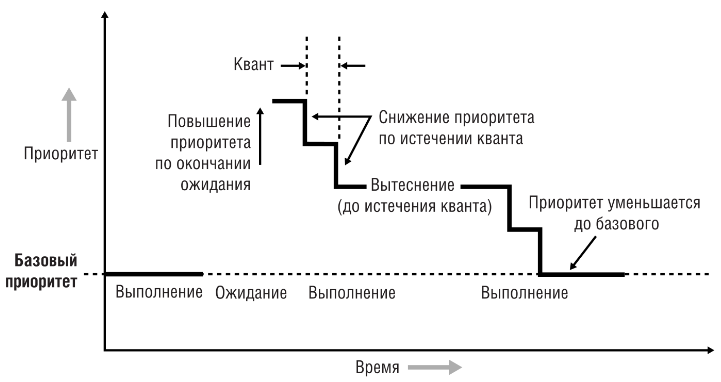
\includegraphics[width=\linewidth]{img/screenshot001}
	\caption{Изменение приоритета}
	\label{fig:1}
\end{figure}

\subsection{Повышение приоритета по окончании ожидания на событии или семафоре}

Если ожидание потока на событии системы или семафоре успешно завершается из-за вы SetEvent, PulseEvent или ReleaseSemaphore, его приоритет повышается на 1. Такая регулировка позволяет равномернее распределить процессорное время -- потокам, блокируемым на событиях, процессорное время требуется реже, чем остальным. В данном случае действуют те же правила динамического повышения приоритета.

К потокам, пробуждающимся в результате установки события вызовом функций NtSetEventBoostPriority и KeSetEventBoostPriority, повышение приоритета применяется особым образом.

\subsection{Повышение приоритета по окончании ожидания потоками активного процесса}

Если поток в активном процессе завершает ожидание на объекте ядра, функция ядра KiUnwaitThread повышает его текущий приоритет на величину значения PsPrioritySeparation. PsPrioritySeparation -- это индекс в таблице квантов, с помощью которой выбираются величины квантов для потоков активных процессов. Какой процесс является в данный момент активным, определяет подсистема управления окнами.

Приоритет повышается для создания преимуществ интерактивным приложениям по окончании ожидания, в результате чего повышаются шансы на возобновление потока приложения. Важной особенностью данного вида динамического повышения приоритета является то, что он поддерживается всеми системами Windows и не может быть отключен даже функцией SetThreadPriorityBoost.

\subsection{Повышение приоритета при пробуждении GUI-потоков}

Приоритет потоков окон пользовательского интерфейса повышается на 2 после их пробуждения из-за активности подсистемы управления окнами. Приоритет повышается по той же причине, что и в предыдущем случае, -- для увеличения отзывчивости интерактивных приложений.

\subsection{Повышение приоритета при нехватке процессорного времени}

Раз в секунду диспетчер настройки баланса -- системный поток, предназначенный для выполнения функций управления памятью -- сканирует очереди готовых потоков и ищет потоки, которые находятся в состоянии готовности в течение примерно 4 секунд. Диспетчер настройки баланса повышает приоритет таких потоков до 15. Причем в Windows 2000 и Windows XP квант потока удваивается относительно кванта процесса, а в Windows Server 2003 квант устанавливается равным 4 единицам. По истечении кванта приоритет потока снижается до исходного уровня. Если потоку все еще не хватило процессорного времени, то после снижения приоритета он возвращается в очередь готовых процессов. Через 4 секунды он может снова получить повышение приоритета.

Чтобы свести к минимуму расход процессорного времени, диспетчер настройки баланса сканирует только 16 готовых потоков за раз, а повышает приоритет не более чем у 10 потоков за раз. Диспетчер настройки баланса не решает всех проблем с приоритетами потоков, однако позволяет потокам, которым не хватает процессорного времени, получить его.

\chapter*{Выводы}

Несмотря на то, что Windows и UNIX разные операционные системы, обработчики прерывания от системного таймера в этих системах выполняют схожие функции:

\begin{itemize}
	\item инициализируют отложенные действия (такие как пересчет приоритетов);
	\item выполняют декремент счетчиков тиков;
	\item уменьшают квант процессорного времени, выделенного процессу.
\end{itemize}

Обе операционные системы являются системами разделения времени с вытеснением и динамическими приоритетами.

Приоритет пользовательского процесса в ОС UNIX может пересчитываться в зависимости от фактора любезности, p\_cpu и базового приоритета. Приоритеты ядра являются фиксированными величинами.

При создании процесса в Windows, ему назначается приоритет, который является базовым относительно приоритетов потоков. Приоритет потока пользовательского процесса может быть пересчитан.

В любой системе у процесса базовый приоритет. Классическое ядро Unix не было многопоточным. Современные ядра и ядра Linux многопоточные.
